\documentclass[oneside]{labbook}

\usepackage[bottom=10em]{geometry} % Reduces the whitespace at the bottom of the page so more text can fit
\usepackage{amsmath} % For typesetting math
\usepackage{graphicx} % Required for including images
\usepackage{lipsum}
\usepackage[english]{babel} % English language
\usepackage[utf8]{inputenc} % Uses the utf8 input encoding
\usepackage[T1]{fontenc} % Use 8-bit encoding that has 256 glyphs
\usepackage[osf]{mathpazo} % Palatino as the main font
% \linespread{1.1}\selectfont % Palatino needs some extra spacing, here 5% extra
\usepackage[nouppercase,headsepline]{scrpage2} % Provides headers and footers configuration
\usepackage{booktabs,array} % Packages for tables
\usepackage{enumitem}

\newcommand{\obj}[1]{\textbf{Objective:} #1\\}
\newcommand{\commit}[1]{\footnote{Git commit \texttt{#1}}}
\newcommand{\reaction}[4][]{
  \begin{equation}
  #2 \overset{#4}{\rightarrow} #3
  \end{equation}}
\newcommand{\lreaction}[4]{
  \begin{equation}
  #2 \overset{#4}{\rightarrow} #3
  \end{equation}}

\DeclareFixedFont{\textcap}{T1}{phv}{bx}{n}{1.5cm} % Font for main title: Helvetica 1.5 cm
\DeclareFixedFont{\textaut}{T1}{phv}{bx}{n}{0.8cm} % Font for author name: Helvetica 0.8 cm
%------------------------------------------------------------------------------
%	DEFINITION OF EXPERIMENTS
%------------------------------------------------------------------------------
\newexperiment{gillespie}{Gillespie algorithm proof-of-concept}
\newexperiment{conjug}{Plasmid conjugation simulation}
%------------------------------------------------------------------------------


\begin{document}
%-------------------------------------------------------------
% Title
%-------------------------------------------------------------
\title{
  \textcap{Laboratory Notebook \\[1cm]
  \textaut{Beginning 05-29-2016}}
}

\author{
  \textaut{JD Russo}\\ \\
  Bucknell University
}

\date{}

\maketitle

\printindex
\tableofcontents
% \newpage

\pagestyle{scrheadings}
%-------------------------------------------------------------


%-------------------------------------------------------------
% Begin journal entries
%-------------------------------------------------------------
\labday{June 1, 2016}
\obj{Refine Gillespie algorithm proof-of-concept, and continue background research.}

\experiment{gillespie}
After reviewing my first version of my code\commit{4105445}, JJ had
feedback on some changes to make, which I'll go through and fix one by one.

\begin{itemize}
  \item[$\Rightarrow$] $\tau$ should be generated with a different random number than the number used
  for determining the reaction.
  \item Changed $\tau$ to use a new, freshly generated number.

  \item[$\Rightarrow$] An unnecessary division in the code when calculating the
  propensity array can be removed for efficiency.
  \item Removed the unnecessary division and timed execution with and without
  using the \texttt{time} command. Too much variation in execution times to determine
  any significant change.

  \item[$\Rightarrow$] How would I modify the array of propensity functions if,
  for example, reaction 2 were changed from $X \rightarrow 2X$ to $2X \rightarrow 3X$?
  Reactions like this can be found in sexual reproduction and chemical reactions.
  \item I need to look into this more. My first guess would be maybe I need to
  square the propensity or probability of that reaction, since two reagents are involved.
\end{itemize}

Before I spend more time trying to answer the last point, I'm going to review some
more background materials. I'll start by reading the Wikipedia page on antimicrobial
resistance, and go from there.

%-------------------------------------------------------------
\labday{June 2, 2016}

\obj{Continue background research on antimicrobial resistance and plasmids.}

\section{Background}
\subsection*{Antimicrobial Resistance}

\begin {itemize}[label={--}]
\item Broader topic than just bacteria and antibiotics
\item 3 primary ways resistance arises in bacteria
\begin{itemize}
  \item Natural resistances
  \item Genetic mutation
  \item Acquiring resistance from another species \textbf{What we're studying with plasmids}
\end{itemize}
\item All classes of microbes develop resistances
\item Present in all parts of the world
\end{itemize}


\subsection*{Mutation}
\begin{itemize}
  \item Low probability of mutating resistances
  \item Some mutations can produce enzymes that render antibiotics inert
  \item Some mutations can eliminate the targets of certain antibiotics
\end{itemize}


\subsection*{Acquired Resistances}
\begin{itemize}
  \item \textit{Conjugation} is passing genetic material from one bacteria to another via
  \textbf{plasmids} and \textbf{transposons}. This requires physical contact
  \item \textit{Transformation} is when a bacteria absorbs genetic material from
  a free plasmid in its environment
  \item Viruses can also take genetic material from a bacterium and inject it into other bacteria
  \item \textbf{Horizontal} transfer is sharing genetic material with other bacteria
  \item \textbf{Vertical} transfer is sharing genetic material through reproduction with daughter cells
  \item \textbf{Transposons} are small amounts of DNA that can move between genetic
  elements like chromosomes and plasmids.
\end{itemize}


\subsection*{Plasmids}
\begin{itemize}
  \item Cannot reproduce on their own, without a host bacterium
  \item Widely distributed
  \item Bacteria can hold many plasmids per cell
  \item Plasmid genomes have \textit{core} genes for transmission and replication
  and \textit{accessory} genes that encode traits.
\end{itemize}


\subsection*{The Plasmid Paradox}
"Plasmids impose a fitness cost on their bacterial hosts that generates selection
against plasmid carriage under conditions in which plasmid genes do not provide
any benefit to the host ... The great irony of the plasmid paradox is that exposure
to conditions that select for plasmid-carried genes can also ultimately lead to
plasmid loss."
\begin{itemize}
  \item Recurrent horizontal transfer
  \item Genes encoded
\end{itemize}

\section*{Skype with Prof. Dong}
\begin{itemize}
  \item For the $2X \rightarrow 3X$ reaction mentioned in yesterday's entry, the
  propensity array element for the new reaction must be multiplied by two. Since
  it involves two reagents now, it's twice as probable. \textit{(Why doesn't this
  make it half as probable?)}

  \item The theoretical line should follow the solution to the ODE, which in the
  simplest case is just the exponential.

  This should be plotted on a semi-log
  plot (meaning logarithmic y-axis) since it's an exponential function. The slope
  of this line will be the exponent.

  \item It would be helpful to average the five independent Gillespie algorithm
  runs that are executed, and compare the average line to the theoretical line.

  However, the Gillespie algorithm has an element of randomness in the time steps
  it takes. Therefore, between separate runs, times of datapoints will not line up.
  Without having points with the same time, we can't meaningfully average them.
  We're not sure what the answer is to this yet, but we're putting it on hold for now.

  We also discussed the central limit theorem, and how if you increase the population
  size in the simulation, the simulation runs become far closer to the theoretical
  model. As the population grows, the standard deviation of the mean is reduced,
  and the Gaussian that describes the distribution of the runs gets narrower.

  In biology, the opposite is often the case, where very small populations lead
  to wide Gaussians, and much noisier data. For example, in our research, if a parent
  cell has 5 plasmids and produces two daughters, it's likely that the plasmids
  will be distributed 3 to one, 2 to the other. However, that's just likely, not
  guaranteed. If this doesn't happen, and if for example one daughter receives all
  5 and the other none, this small initial difference can hugely affect the system
  as it grows.

  \item We would like to start discussing a journal article every week to become
  more familiar with the literature surrounding this topic. To that end, I've
  been provided with a first article to read\cite{thattai}.

  \item We talked a little about the background research I had done, and a little
  more in depth about a few of the topics I'd read on. We talked about how
  cells can lose plasmids without dying, releasing them back into their
  environment.

  \item Finally, we discussed next steps for simulation.
\end{itemize}


\subsection*{Next Steps}

Currently\commit{5932c50}, the simulation only models the following two reactions

% \reaction{X}{\emptyset}{\mu_1}
% \reaction{X}{2X}{\mu_2}
\begin{align}
  X & \overset{\alpha}{\rightarrow} \emptyset\\
  X & \overset{\mu_2}{\rightarrow} 2X
\end{align}
which correspond to death and reproduction respectively. However, in order to
move forward, we'd like to expand the reactions considered.

\subsubsection{Theory}

We can simulate a bacterium transforming by taking in a plasmid from its
environment with a new set of reactions

% \lreaction{xbirth}{X}{2X}{\mu_1}
% \lreaction{transform}{X}{Y}{\alpha}
% \reaction{Y}{2Y}{\mu_2}

\begin{align}
  X & \overset{\mu_1}{\rightarrow} 2X \label{rxn:x_birth}\\
  X & \overset{\alpha}{\rightarrow} Y \label{rxn:transf}\\
  Y & \overset{\mu_2}{\rightarrow} 2Y \label{rxn:y_birth}
\end{align}

where X is a bacterium that has not absorbed any plasmids and Y is a plasmid
carrier. Eqn. \ref{rxn:transf} represents transformation, the
process by which a bacterium takes a free plasmid from its environment.

From this, we can quickly see that as per the plasmid paradox mentioned before,
$\mu_1 > \mu_2$. In addition, we can determine the cost to fitness of owning a
plasmid to be
\begin{equation}
\frac{\mu_1}{\mu_2}.
\end{equation}

However, the ratio of X to Y will depend significantly on $\alpha$, the probability
of transformation. We can rewrite the above reactions as differential equations

\begin{align}
  \frac{dX}{dt} & = \mu_1 \text{X} - \alpha \text{X} \label{eq:x_pop}\\
  \frac{dY}{dt} & = \mu_2 \text{Y} + \alpha \text{X} \label{eq:y_pop}
\end{align}
that describe the growth of each population. These have analytical results, but
may be manipulated into a form that has an exact solution. I'll need to find this
exact solution so I can verify my simulations are producing the proper output.

Once I have the simulation working, I'd like to look at behaviors like how large
$\alpha$ can get before Y dominates X.

In addition, $\alpha$ doesn't have to be
constant, and in fact should depend on plasmid concentration. I will make it into
a function that depends on the plasmid concentration, P.

I'd also like to map the transition of where X and Y dominate. I can do this by
plotting $\frac{\mu_1}{\mu_2}$ vs $\alpha$, and then highlighting regions where
each dominate. This will allow us to explore how X and Y change with $\alpha$.

For now, we will use these 3 reactions and only vary $\alpha$ in order to try
and find the $\frac{\mu_1}{\mu_2}$ vs $\alpha$ relation.

In the future, we'd like to perform this simulation on a lattice to take spatial
configuration of the bacteria into account, but for now we will assume a well-mixed
environment.

\labday{June 3, 2016}

\obj{Prepare short talk for progress talks today, and begin work on second
simulation.}

Every Friday we're asked to give a 3-4 minute presentation to the other summer
research students. I've spent some time putting together my basic talking points,
which can be found in \texttt{summer2016/talks/June\_3.pdf}.

\experiment{conjug}
I'm also starting work on a simulation as mentioned in yesterday's entry, where
I replace the initial two (birth and death) reactions with three, bacteria
reproduction, transformation, and plasmid carrier reproduction.

I've duplicated the code from the initial simulation to
\texttt{summer2016/dev/plasmids.py}, where I'll begin modifying it.

I've redefined the reactions, and made the program keep track of X and Y
(bacteria and carrier) populations separately.

I can plot the results of this simulation, and see that if I increase alpha, the
point where the X and Y populations cross shifts to the left.


\labday{June 6, 2016}

\obj{Expand plasmid carrier population simulation to run through our parameter
space and meaningfully plot results.}

\experiment{conjug}
Our goal with the plasmid carrier population simulation is to be able to make a
plot of $\frac{\mu_1}{\mu_2}$ vs $\alpha$. I think it would make sense to show
this as a contour plot. I can generate a large number of datapoints throughout
the plot, and then plot them indicating whether the X or Y population dominated
(maybe blue-red spectrum?).

Alternatively, I can save the results of each run
(i.e. $\frac{\mu_1}{\mu_2}$, $\alpha$, and X and Y populations) and then do some
interpolation to get a smoother plot, but that may be more effort than it's worth
and I'm not sure that's the results we'd even want.

I've modified the code to generate either a contour plot, or an animation of the
contour plot at different timesteps. These timesteps are currently independent,
i.e. if you run for T = 1, 2, 3  it will not be snapshots of the same simulation
at T=1, 2, and 3. It will be 3 separate, independent simulation runs.

Now that I have my simulation results, I will model what plot I'd expect to see
from the differential equations describing the reactions.

I've modelled $\frac{\mu_1}{\mu_2}$ vs $\alpha$ in Mathematica, using the same
value of $\mu_1 = .8$ and ranges of $\alpha = [.2 .. ,7]$ and $\mu_2 = [.29 ... .8]$.
However, the contour animation in Mathematica does not seem to show the Y population
dominating the X as quickly as the simulation does. Examples at $T=0.9$ and
$T=1.5$ are provided below.


\begin{figure}[h!]
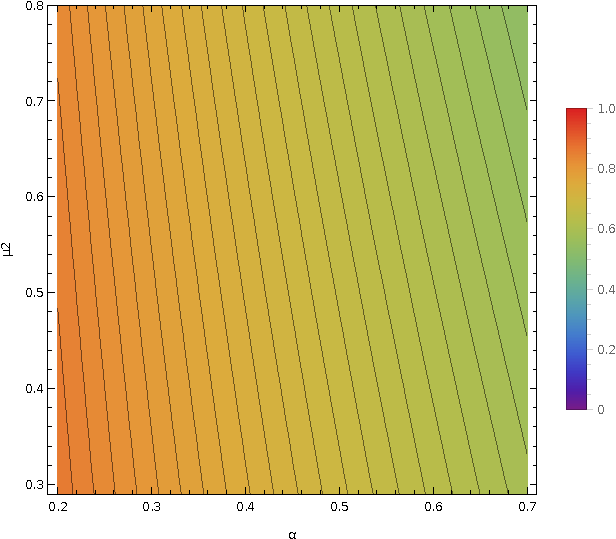
\includegraphics[width=.5\columnwidth]{mathematica_T0_9.pdf}
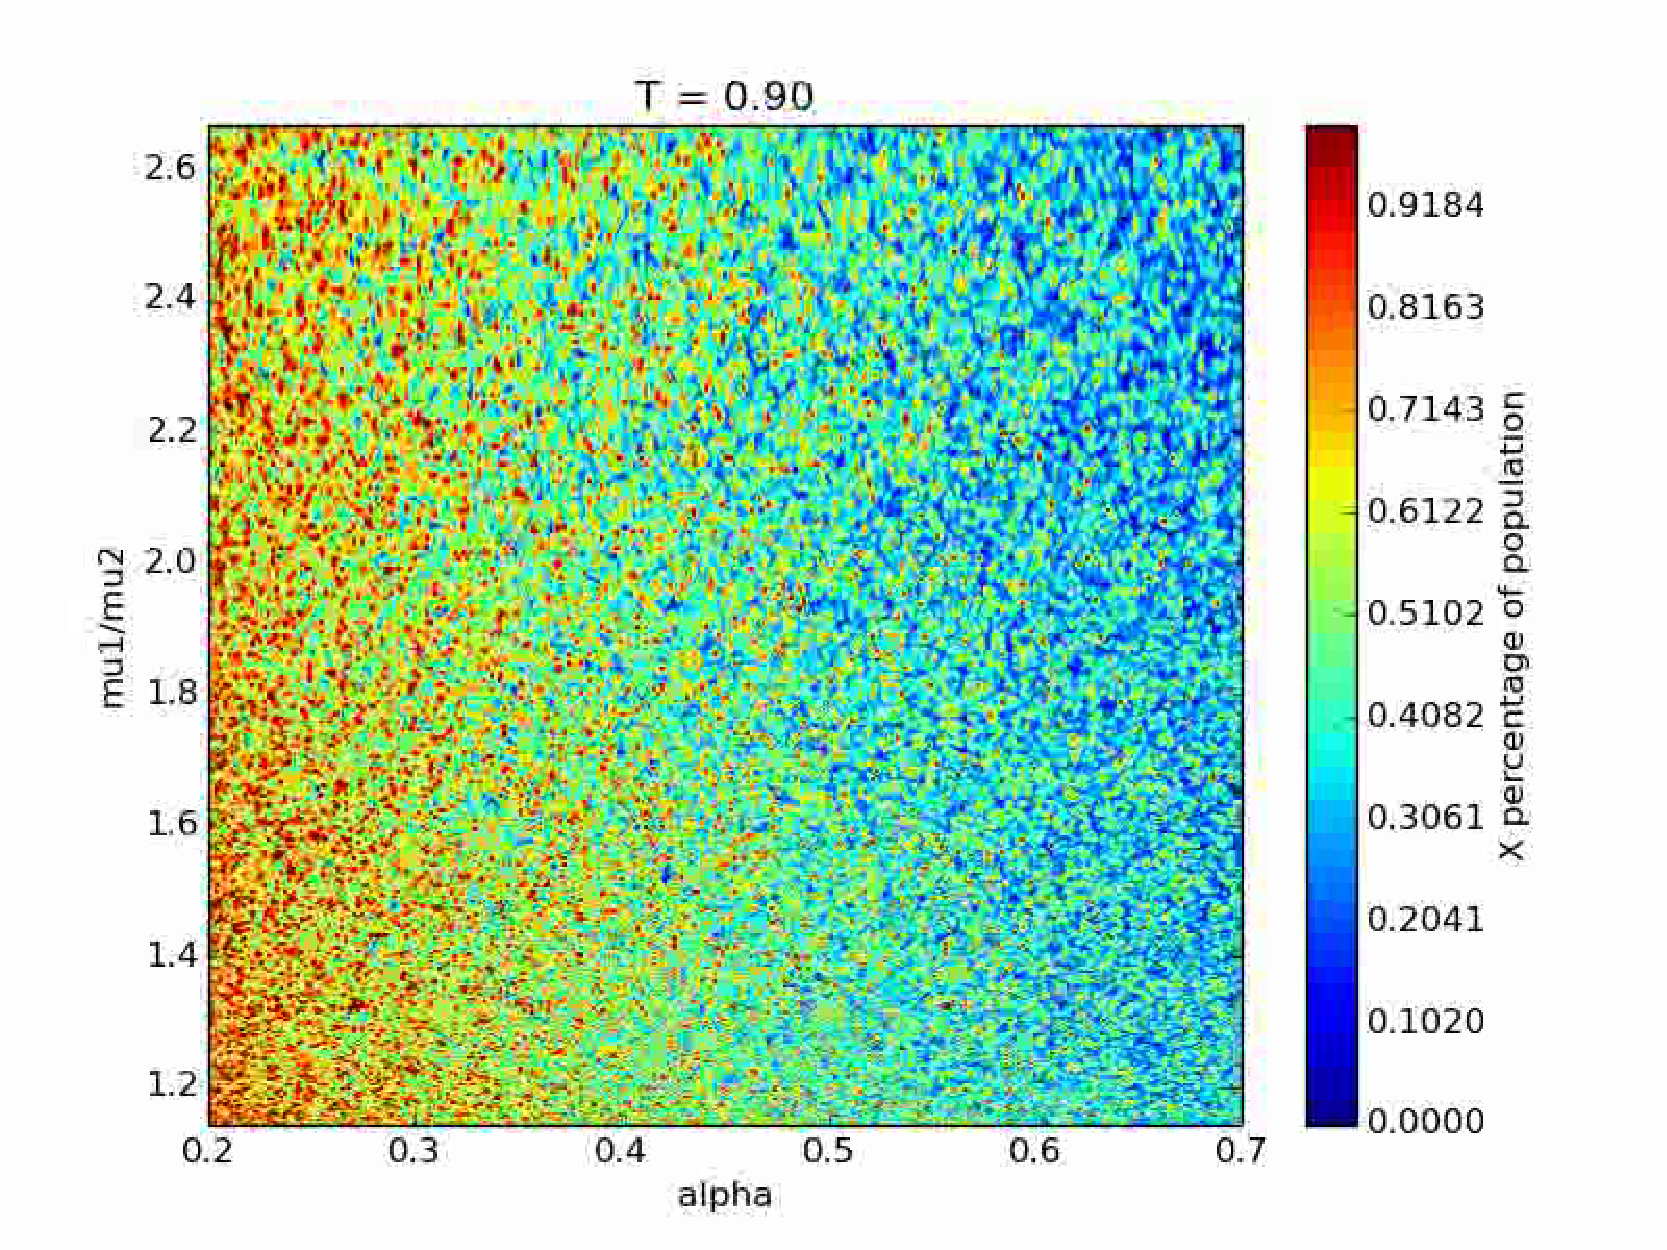
\includegraphics[width=.5\columnwidth]{python_T0_9.pdf}
\caption{Plots of $\mu2$ vs $\alpha$ at $T=0.9$ in Mathematica (left) and Python (right)}
\end{figure}

\begin{figure}[h!]
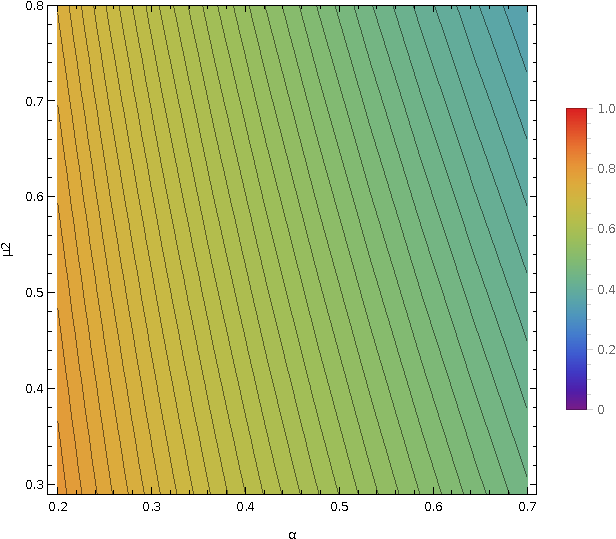
\includegraphics[width=.5\columnwidth]{mathematica_T1_5.pdf}
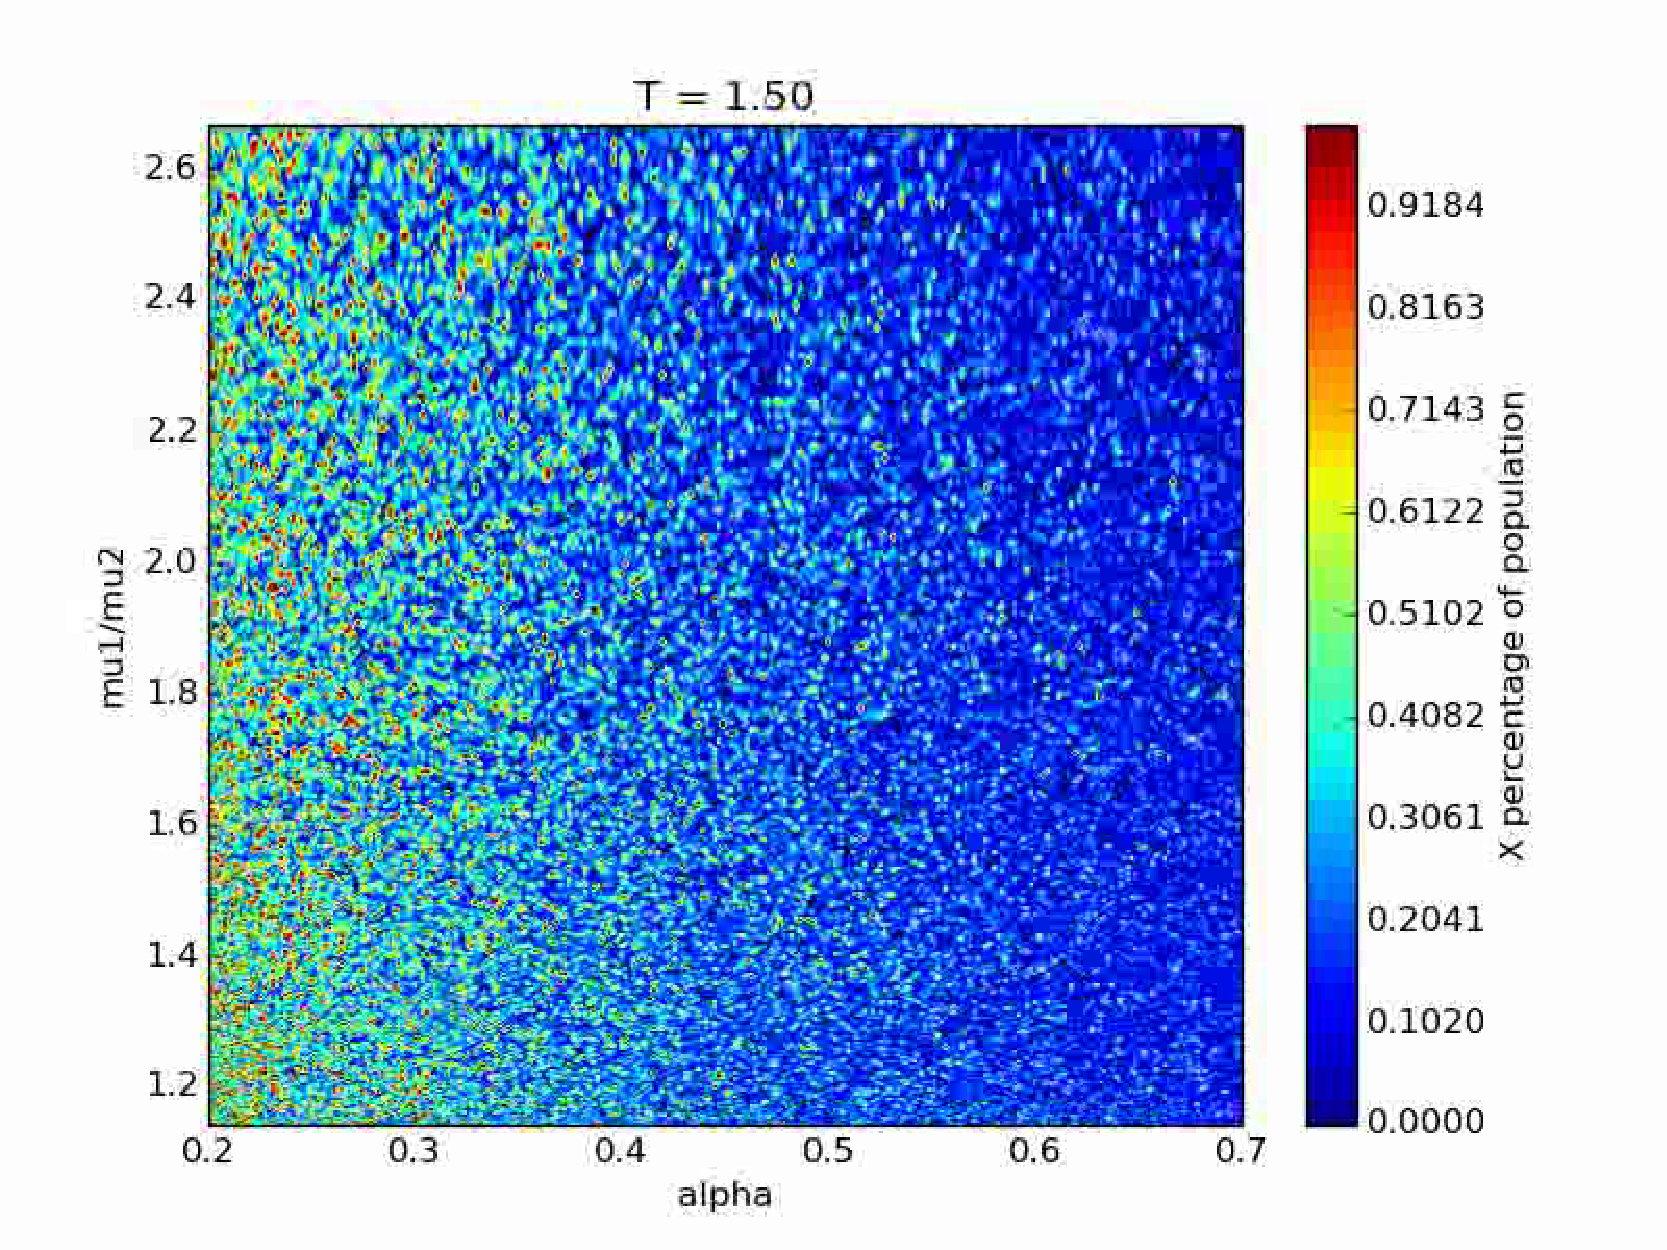
\includegraphics[width=.5\columnwidth]{python_T1_5.pdf}
\caption{Plots of $\mu2$ vs $\alpha$ at $T=1.5$ in Mathematica (left) and Python (right)}
\end{figure}

These figures are a little hard to compare though, because the color schemes
aren't quite the same. I'll work on finding a way to match those up, or perhaps
revisit the interpolated contour plot I have in \texttt{plasmids.py}. Using that,
I could label the contours on both, and compare values that way.


\labday{June 7, 2016}

\obj{Present simulation results to JJ, and consider next steps.}

\experiment{conjug}
I've added \texttt{animate2} and \texttt{animate3} function to animate an
interpolated contour plot and a 3D surface plot, respectively.

The code will occasionally error if one population goes to zero - handle that
more gracefully!

\labday{June 8, 2016}

\obj{Derive equations for susceptible and resistant population growths, and
compare to my results from Mathematica.}

We start with the equations
\begin{align}
  \frac{dS}{dt} & = b_S S - \alpha S \label{eq:S_growth}\\
  \frac{dR}{dt} & = b_R R + \alpha S \label{eq:R_growth}
\end{align}
describing two populations of particles, S and R, where $b_S$ is the birth rate
of the S (susceptible) population, $b_R$ is the birth rate of the R (resistant)
population, and $\alpha$ is the rate at which an S particle can acquire a plasmid
and become an $R$. These are similar to equations
\eqref{eq:x_pop} and \eqref{eq:y_pop} mentioned earlier. My goal is to obtain an
exact solution for $S(t)$ and $R(t)$.

By rewriting \eqref{eq:S_growth} as
\begin{equation*}
\frac{dS}{dt} = \left( b_S - \alpha \right) S
\end{equation*}
one can see that there is a solution of the form
\begin{equation}\label{eq:S_sol}
S(t) = S_0\:e^{\left(b_S - \alpha\right) t}.
\end{equation}


\begin{align*}
  \frac{dR}{dt} &= b_R R + \alpha S  &&
      \text{Substitute in \eqref{eq:S_sol} for S.} &\\[1.25ex]
  \frac{dS}{dt} &= \left( b_S - \alpha \right) S &&
      \text{Set } R(t)=y(t)e^{\mu t} \text{ and } \mu = b_S - \alpha. &\\[1.25ex]
  \mu y(t) e^{\mu t} + \dot{y}(t) e^{\mu t} &= b_R y(t) e^{\mu t} + \alpha S_0 e^{\mu t} &&
      \text{Simplify.} &\\[1.25ex]
  \mu y(t) + \dot{y}(t) &= b_R y(t) + \alpha S_0 &&
      \text{Solve for } \dot{y}. &\\[1.25ex]
  \dot{y}(t) &= (b_R - \mu) y(t) + \alpha S_0 &&
      \text{Set } a = (b_R - \mu) \text{ and } b = \alpha S_0. &\\[1.25ex]
  \dot{y}(t) &= a y(t) + b &&
      \text{Let } x = \dot{y}. &\\[1.25ex]
  x &= ay + b &&
      \text{Take the derivative }\dot{x}. &\\[1.25ex]
  \dot{x} &= a \dot{y} &&
      \text{Substitute in } \dot{y} = x. &\\[1.25ex]
  \dot{x} &= a x &&
      \text{Write the general solution to } x.&\\[1.25ex]
  x(t) &= x_0 e^{a t} &&
      \text{Expand.} &\\[1.25ex]
\end{align*}

\begin{align*}
  x_0 e^{(b_R - \mu) t} &= ay + b&&
      \text{Solve for } y &\\[1.25ex]
  y &= \frac{1}{b_R - \mu} \left(x_0 e^{(b_R - \mu)t} - \alpha S_0\right) &&
      \text{Substitute back to get an expression for } R(t). &\\[1.25ex]
  R(t) &= \frac{e^{\mu t} }{b_R - \mu} \left( x_0 e^{(b_R - \mu)t} - \alpha S_0 \right) &&
      \text{Simplify.} &\\[1.25ex]
  R(t) &= \frac{1}{b_R + b_S + \alpha} \left[ x_0 e^{b_R t} - \alpha S_0 e^{(b_S - \alpha)t} \right]&&
      \text{To determine $x_0$, first solve for $R(0)$,} &\\[1.25ex]
  R(0) &= \frac{1}{b_R + b_S + \alpha} \left[ x_0 - \alpha S_0 \right] &&
      \text{\quad then solve for } x_0. &\\[1.25ex]
  x_0 &= (b_R - b_S + \alpha) R(0) + \alpha S_0 &&
      \text{Plug back in to R(t) and simplify.} &\\[1.25ex]
  R(t) &= R_0 e^{b_R t} + \frac{\alpha S_0}{b_R - b_S + \alpha} \left(e^{b_R t} - e^{(b_S - \alpha)t} \right) &&
      \textbf{Exact equation for $R(t)$.} &\\[1.25ex]
\end{align*}

This is consistent with my results from Mathematica.

\labday{June 9, 2016}

\section*{Skype with Prof. Dong}
\begin{itemize}
\item We discussed that it would be more useful to view absolute S population, rather
than plotting a relative percentage.
\item It'd be useful to characterize fluctuations by plotting trajectories for
$X_0 = 1000$, $X_0 = 1000000$, and the model.
\item We'd like to look at longer timescales, to see how long until X dies out
or until Y dominates. The issue with this is the time it takes to run longer
simulation.
\item The X death timescale should be $\mu_1 - \alpha$.
\item We'd like to use a Hill function for $\alpha$ to add some dependence on
$X_0$, since realistically the number of available plasmids would decrease as
the population increases and uses them up.
\item Michaelis-Menten kinetics are used to relate reaction rates to substrate
concentration. This is essentially what we'd be doing with Hill functions and
alpha. (Are we doing the reverse, relating reaction rate to reactant concentration?)
\item We'd also like to calculate equilibrium conditions for S and R populations
(see Michaelis-Menten equilibrium approximation)
\vspace{9mm}
\item In bacteria populations, the \textbf{carrying capacity} of the environment
determines the upper limit on the population -- we'd like to include this.
\item This would change the DE for population growth to
\begin{equation}
\frac{dS}{dt} = b_s \left( 1 - \frac{(S+R)}{k}\right) - \alpha S
\end{equation}
where $k$ is the environment's carrying capacity, the maximum number of individuals
it can sustain. This is logistic growth.
\item $\frac{dS}{dt} = b_s \left( 1 - \frac{(S+R)}{k}\right) - \alpha S$ has
solutions at $S=0,k$. If we start somewhere in between, what determines which
equilibrium point we will go to?
\item We can see this with Kinetic Monte Carlo by doing time traces at
different $X_0$s and seeing which solution it goes to.
\vspace{9mm}
\item We'd also like to incorporate a death rate, and calculate the equilibrium
point with that.
\end{itemize}

\labday{June 13, 2016}
\obj{Refactor code to work more reliably, intuitively, and efficiently.}

The first version of \texttt{plasmids.py}\commit{bd8b069} did not accurately
track one population of bacteria to explore time evolution
of a system. Instead, it would do an independent simulation to each time step,
and plot the results of that. We don't want that, we want to track one simulation
to examine the dynamics in it, so I factored that in when rewriting.

I've committed my rewrite\commit{3034cd6}, which addresses this issue in addition
to making a slightly cleaner method for plotting data.

\labday{June 13, 2016}

\section*{Skype with Prof. Dong}
We began by reviewing some of my generated plots, and detailing how we could
improve them.
% \begin{itemize}
% \end{itemize}

\obj{Use equations for $S(t)$ and $R(t)$ to find when $S=R$. This will help
us find an interesting parameter range to use.}

By setting $\frac{S(t)}{R(t)}=1$ and solving for $t$, we can find that the
crossover time where $R=S$ is given by
\begin{equation}
t = \frac{1}{b_R - b_S + \alpha} \ln\left( \frac{b_R - b_S + 2 \alpha}{\alpha}\right).
\end{equation}

This can be analyzed to find interesting parameter ranges, where the crossover
time is within the time spans we're looking at. Until now, I've typically been
using values of $\mu_1=0.8$, $\mu_2=.7 { to } .78$ and $\alpha=0.1 { to } 0.1$.
However, these yield a crossover time of $32.4 - 5$. This is much longer than
I've let my simulations run (because of time constraints), and so I would've
never seen this behavior.

By changing $\alpha$ to $.1 \text{ to } .3$ this time scale changes to
 $t = 9.33 \text{ to } 2.55$, a more reasonable value that is within the timescales
we're looking at.

\experiment{conjug}
\subsection*{Multiprocessing}
As we start to move up to more combinations of parameters, longer timesteps,
and more simulation runs, computation time becomes much more important.

In order to make the simulation a little faster, I've implemented
multiprocessing\commit{2380518f}.
So, when combinations of parameters are run, the program will break off each
Gillespie algorithm run to its own process.\\

\begin{tabular}{l|c|c|c|r|r|}
  \hline
System & Parallelized & $S_0$ & $T_max$ & Runtime(s) & Gillespie Runs\\
\hline
Local & Y & 100 & 10 & 00.64, 00.59, 00.52, 00.57 & 1\\
Local & Y & 100 & 15 & 09.17, 12.55, 09.40, 08.94 & 1\\
Local & Y & 100 & 16 & 16.82, 14.85, 18.12, 18.85 & 1\\
Local & Y & 100 & 17 & 45.51, 31.73, 37.71, 38.26 & 1\\
Local & Y & 100 & 18 & 71.21, 79.51  & 1\\
\hline
Remote & Y & 100 & 16 & 64.392 & 9\\
Local & Y & 100 & 16 & 240 & 9\\
Local & N & 100 & 16 & 757 & 9\\
\hline
\end{tabular}

Not shown, the linux remote is roughly 1/2 as fast for a single run as my local
system.

\labday{June 20, 2016}

\begin{itemize}
\item Added plots of R population
    * Now focusing mostly on X vs T, have found interesting param range
\item Added some sanity checks in code for making sure the populations are positive before
  removing members from them.
\item Changed from log base $e$ to log10
\end{itemize}

\labday{June 28, 2016}

\obj{Clean up results and prepare presentation quality visualizations of
data from simulation.}

I'm essentially done with the code for simulating the well-mixed case, so I'm
going to take some time to collect my results from the simulation. I will be
collecting data and plots of population vs time of both asymmetric and symmetric
cases for the following:
\begin{itemize}
  \item Constant $\alpha$
  \item Linear $\alpha$
  \item Recycling $\alpha$
\end{itemize}
I'd also like to add code to plot the total number of plasmids.

The plots for recycled and constant alpha seem the same.



\labday{June 29, 2016}

\obj{Separate plotting code from simulation code}




\labday{June 30, 2016}

\obj{Begin planning for simulation on a lattice}


\labday{July 8, 2016}

\obj{Write differential equations for the linear $\alpha$ and recycled $\alpha$
cases.}

We can write the differential equations governing the S and R populations with a
constant transformation rate $\alpha$, S and R birthrates $\mu_1$ and $\mu_2$,
R death rate $\delta$ and a carrying capacity $K$ using the following equations:
\begin{align}
\frac{dS}{dt}& = \mu_1 \left(1 - \frac{S + R}{K}\right)S - \alpha S \\
\frac{dR}{dt}& = \mu_2 \left(1 - \frac{S + R}{K}\right)R + \alpha S - \delta R
\end{align}

In order to model a population with an initial fixed number $P_0$ of available
plasmids and a linear dependence of $\alpha$ on number of available free plasmids,
a third equation must be added to model the number of plasmids. The first two
equations must also be revised.

\begin{align}
  \frac{dS}{dt} & = \mu_1 \left(1 - \frac{S + R}{K}\right)S - \alpha
  \left( \frac{P}{P_0} \right) S \\
\frac{dR}{dt} & = \mu_2 \left(1 - \frac{S + R}{K}\right)R + \
  \alpha S  \left( \frac{P}{P_0} \right) - \delta R \\
\frac{dP}{dt} & = -\alpha P
\end{align}

These all assume symmetric divison for R cells, in other words that
$R \rightarrow 2R$. However, to conserve number of plasmids, this reaction is
actually the asymmetric: $R \rightarrow S + R$. To include this in the equations
for the S and R populations, a term must be moved from the R to S equation.

\begin{align}
  \frac{dS}{dt} & = \mu_2 \left(1 - \frac{S + R}{K}\right)R +
  \mu_1 \left(1 - \frac{S + R}{K}\right)S - \alpha
  \left( \frac{P}{P_0} \right) S \\
\frac{dR}{dt} & =  \alpha S  \left( \frac{P}{P_0} \right) - \delta R \\
\frac{dP}{dt} & = -\alpha P
\end{align}


%------------------------------------------------------------------------------
%	BIBLIOGRAPHY
%------------------------------------------------------------------------------
\begin{thebibliography}{2}
% \bibitem{lamport94}
% Leslie Lamport,
% \emph{\LaTeX: A Document Preparation System}.
% Addison Wesley, Massachusetts,
% 2nd Edition,
% 1994.
\bibitem{thattai}
Mukund Thattai, Alexander van Oudenaarden
\emph{Intrinsic noise in gene regulatory networks}
PNAS vol. 98 no. 15
2001.
http://www.pnas.orgycgiydoiy10.1073ypnas.151588598/
\end{thebibliography}
%------------------------------------------------------------------------------

\end{document}
